\documentclass[9pt]{beamer}

%!TEX root = ../notas_de_clase.tex

%preamble

%language
\usepackage[spanish,es-nodecimaldot]{babel}
\usepackage[utf8]{inputenc}
\usepackage{apacite}
\usepackage[absolute,overlay]{textpos}

%packages
\usepackage[Algoritmo]{algorithm}
\usepackage{algorithmicx}
\usepackage[noend]{algpseudocode}
\usepackage{mathtools}
\setlength {\marginparwidth}{2cm}
\usepackage{todonotes}
\usepackage{amsbsy}
\usepackage{amssymb}
\usepackage{amsmath,bm}
\usepackage{dsfont}

\usepackage{xcolor}
\providecommand{\sred}[1]{\textcolor{red}{#1}}
\providecommand{\sblue}[1]{\textcolor{blue}{#1}}
\providecommand{\red}[1]{\textcolor{red}{\text{#1}}}
\providecommand{\blue}[1]{\textcolor{blue}{\text{#1}}}
\providecommand{\redb}[1]{\textcolor{red}{\textbf{#1}}}
\providecommand{\blueb}[1]{\textcolor{blue}{\textbf{#1}}}
\usepackage{graphicx}
\usepackage{fancybox}
\usepackage{booktabs}
\usepackage{caption}
\usepackage{float}
%\usepackage[longend,ruled,algochapter,linesnumbered,lined,boxed,commentsnumbered,spanish]{algorithm2e}
%\usepackage[algo2e]{algorithm2e}
\usepackage{amssymb}
\usepackage{amstext}
\usepackage{bm}
\usepackage{wrapfig}
\usepackage{subcaption} % para_unsupervised_chapter

%formatting

\usepackage[export]{adjustbox}

%caption para figuras
\captionsetup[figure]{width=.8\linewidth, font=small,labelfont={bf},name={Fig.},labelsep=period}
\captionsetup[table]{width=.8\linewidth,font=small,labelfont={bf},name={Tabla},labelsep=period}



\ifx\byn\undefined
    \definecolor{my_blue}{HTML}{C2D5FF}
    \definecolor{my_red}{HTML}{FFC2C2}
    \definecolor{my_yellow}{HTML}{FFFFE0}
\else
    \definecolor{my_blue}{HTML}{FFFFFF}
    \definecolor{my_red}{HTML}{FFFFFF}
    \definecolor{my_yellow}{HTML}{FFFFFF}
\fi


\usepackage[framemethod=TikZ]{mdframed}
\mdfdefinestyle{discusion}{%
    %linecolor=black,
    %outerlinewidth=0pt,
    roundcorner=0pt,
    innertopmargin=5pt,
    innerbottommargin=5pt,
    innerrightmargin=20pt,
    innerleftmargin=20pt,
    backgroundcolor=my_blue}

\colorlet{Green}{green!90}


\mdfdefinestyle{ejemplo}{%
    %linecolor=black,
    %outerlinewidth=0pt,
    roundcorner=0pt,
    innertopmargin=5pt,
    innerbottommargin=5pt,
    innerrightmargin=20pt,
    innerleftmargin=20pt,
    backgroundcolor=my_yellow}


\mdfdefinestyle{pendiente}{%
    style = discusion, 
    backgroundcolor=my_red}


\RequirePackage{url}



%definitions
\def\td{{\text d}}
\def\cN{{\mathcal N}}
\def\cX{{\mathcal X}} 
\def\cC{{\mathcal C}} 
\def\N{{\mathbb N}}
\def\d{{\text d}}
\def\datos{{\mathcal D}}
\def\eye{{\mathbb I}}
\def\ssum{{\scriptstyle\sum}}
\def\bepsilon{{\bm \epsilon}}
\def\tx{\tilde{x}}
\def\tX{\tilde{X}}
\def\thetaMAP{\theta_\text{MAP}}
\newcommand{\gp}{\ensuremath{\mathcal{GP}}}
\newcommand{\pr}{\ensuremath{\mathbb{P}}}
\newcommand{\x}{\ensuremath{\mathbf{x}}}
\newcommand{\z}{\ensuremath{\mathbf{z}}}
\newcommand{\cvector}{\ensuremath{\mathbf{c}}}
\newcommand{\e}{\ensuremath{\mathbf{e}}}
\newcommand{\y}{\ensuremath{\mathbf{y}}}
\newcommand{\bx}{\ensuremath{\textcolor{blue}{X}}}
\newcommand{\by}{\ensuremath{\textcolor{blue}{Y}}}
\newcommand{\rx}{\ensuremath{\textcolor{red}{X_*}}}

\newcommand{\R}{\mathbb{R}}
\newcommand{\norm}[1]{\left\lVert#1\right\rVert}




\DeclareMathOperator*{\argmax}{arg\,max}
\DeclareMathOperator*{\argmin}{arg\,min}
\DeclareMathOperator{\E}{\mathbb{E}}
\DeclareMathOperator{\V}{\mathbb{V}}
\DeclareMathOperator{\KL}{\text{KL}}
\DeclareMathOperator{\MVN}{\text{MVN}}
\newcommand\deq{\stackrel{\mathclap{\normalfont\mbox{\tiny def}}}{=}}
%\newcommand{\E}[1]{\mathbb E \left[#1\right]}
\newcommand{\trace}[1]{\text{Tr} \left[#1\right]}


\usepackage{amsthm}

%-------------------------------------------
% Newtheorem
%-------------------------------------------
\newtheorem{axioma}{\textcolor{red}{Axioma}}
\newtheorem{definicion}{Definición}
\newtheorem*{notacion}{Notación}
\newtheorem{teorema}{Teorema}
\newtheorem{corolario}{Corolario}
\newtheorem{lema}{Lema}
\newtheorem{lemaZ}{\textcolor{red}{Lema}}
\newtheorem{propiedad}{Propiedad:}
\newtheorem{proposicion}{Proposición:}
\newtheorem*{observacion}{Observación}
\newtheorem*{comentario}{Comentario}
\newtheorem*{ejemplo}{Ejemplo}
\newtheorem*{resultado}{Resultado}
\newtheorem*{propuesto}{Ejercicio propuesto}
\newtheorem*{demostracion}{Demostración} % No se usa, usar \begin{proof}\end{proof} que son por default.

%listing paackage para código
\usepackage{listings}
\usepackage{xcolor}
 
\definecolor{codegreen}{rgb}{0,0.6,0}
\definecolor{codegray}{rgb}{0.5,0.5,0.5}
\definecolor{codepurple}{rgb}{0.58,0,0.82}
\definecolor{backcolour}{rgb}{0.95,0.95,0.92}
 
\lstdefinestyle{mystyle}{
    xleftmargin=0.15\textwidth,
    linewidth=0.8\textwidth,
    backgroundcolor=\color{backcolour},   
    commentstyle=\color{codegreen},
    keywordstyle=\color{magenta},
    numberstyle=\tiny\color{codegray},
    stringstyle=\color{codepurple},
    basicstyle=\ttfamily\footnotesize,
    breakatwhitespace=true,         
    breaklines=true,                 
    captionpos=b,                    
    keepspaces=true,                 
    numbers=left,                    
    numbersep=5pt,                  
    showspaces=false,                
    showstringspaces=false,
    showtabs=false,                  
    tabsize=2
}
 
\lstset{style=mystyle}

\numberwithin{equation}{section}

\usetheme{simple}

\title{Clase 1 - Introducción}
\subtitle{Aprendizaje de Máquinas - MA5204}
\date{\today}
\author{Felipe Tobar}  
\titlegraphic{
\begin{figure}[htp] 
    \centering
        
\includegraphics[width=0.15\textwidth]{../img/Uchile.pdf}% 
\end{figure}
}
\institute{Department of Mathematical Engineering \&\\ Center for Mathematical Modelling\\Universidad de Chile}

\begin{document}
\begin{frame}
  \titlepage
\end{frame}

\section{Logística y presentación del curso}
\begin{frame}{Organización del curso}

\begin{itemize}
  \item 2 clases por semana de 1 hora: lunes y miércoles de 9 a 10 
  \item Curso sincrónico con asistencia opcional
  \item Clases quedarán disponibles en \href{https://www.youtube.com/channel/UCqtRBEV1r7X4ZbO3089CaaA}{\tt youtube.com/channel/UCqtRBEV1r7X4ZbO3089CaaA}
  \item 7 Evaluaciones a aprobar individualmente 
  \begin{itemize}
    \item 3 tareas de programación en grupos de 2 estudiantes (1/3)
    \item 3 tareas teóricas/conceptuales individuales (1/3)
    \item 1 tarea/proyecto final individual (1/3)
  \end{itemize}
  \item Además de Ucursos, la página con el material del curso es: \href{https://github.com/GAMES-UChile/Curso-Aprendizaje-de-Maquinas}{\tt github.com/GAMES-UChile/Curso-Aprendizaje-de-Maquinas}
  \item Apunte del curso y diapositivas disponible. Material experimental \textbf{que no reemplaza la clase}
  \item Canal de consultas oficial es el foro de Ucursos
\end{itemize}

\end{frame}


\begin{frame}{Objetivos del curso}

\red{Principal:} Conocer y entender las principales herramientas de AM para: 


\begin{itemize}
  \item Saber qué herramienta usar en cada situación 
  \item Identificar sus  ventajas y desventajas en la resolución de un problema particular
  \item Entender los supuestos tomados
  \item Implementarlas en un escenario tanto simulado como real
  \item Continuar estudios que permitan mejorar dichas herramientas 
\end{itemize}
\vfill

Además de los elementos teórico y prácticos, otros objetivos del curso incluyen

 \begin{itemize}
  \item Explicar, en leguanje propio, los conceptos que justifican los metodos vistos  
  \item Presentar de forma clara y concisa sus resultados 
  \item Seguir indicaciones de formato y extensión de reportes de resultados
  \item Poder cumplir las fechas de entrega de las evaluaciones
\end{itemize}

\end{frame}


\begin{frame}{Enfoque y contenidos del curso}

El curso ofrece una perspectiva probabilística al AM, lo cual incluye la presentación de modelos estadísticos como también una interpretación prbabilistica de otros modelos. El foco del curso no son los modelos profundos, pero de todas formas éstos se incluye como contenido en el contexto de la perspectiva del curso.\\
\vspace{2em}
Contenidos:

\begin{enumerate}
  \item Introducción: ¿qué es la Inteligencia Artificial y cómo se relaciona con el AM? 
  \item Regresión
  \item Clasificación
  \item Selección y evaluación de modelos
  \item Máquinas de soporte vectorial
  \item Aprendizaje no supervisado
  \item Redes neuronales
  \item Process Gaussianos 
\end{enumerate}
\vfill


\end{frame}


\begin{frame}{Formato clases y material disponible}


\begin{itemize}
  \item Tendremos 2 clases de 1 hora a la semana, no hay clases auxiliares. 
  \item Se asume dominio de elementos básicos de probabilidades y de programación. Si alguno/a necesita repasar dicho contenidos, se indicará el material para poder hacerlo pero no serán parte de la clase. 
  \item Debido a los perfiles variados de lo/as estudiantes, se espera estudio personal en complemento a las clases. Para lo cual también se indicará las fuentes para hacerlo
  \item Apunte y diapositivas disponible desde el comienzo del curso (en contante mejora)
  \item Tareas y demos disponibles a medida avanza el curso
\end{itemize}
\vfill


\end{frame}


\begin{frame}{Cuerpo docente}

\textbf{Profesor:} Felipe Tobar
\begin{itemize}
  \item Ingeniero Eléctrico (DIE, 2010) 
  \item Areas de Investigación: AM \& procesamiento de señales
  \item Coordinador Master of Data Science 
  \item Investigador: Centro del Modelamiento Matemático 
  \item E-mail: \url{ftobar@dim.uchile.cl}
  \item Website: \href{http://www.dim.uchile.cl/~ftobar/}{\tt dim.uchile.cl/~ftobar/} 
\end{itemize}

\vfill
\textbf{Auxiliares:}
\begin{itemize}
  \item Francisco Vásquez (MSc-DIM)
  \item Fernando Fetis (DIM) 
  \item Nelson Moreno  (DIM) 
  \item Arie Wortsman (DIM) 
  \item Víctor Faraggi (DCC) 
\end{itemize}
\vfill
  \begin{textblock}{7}(14,0.5)
    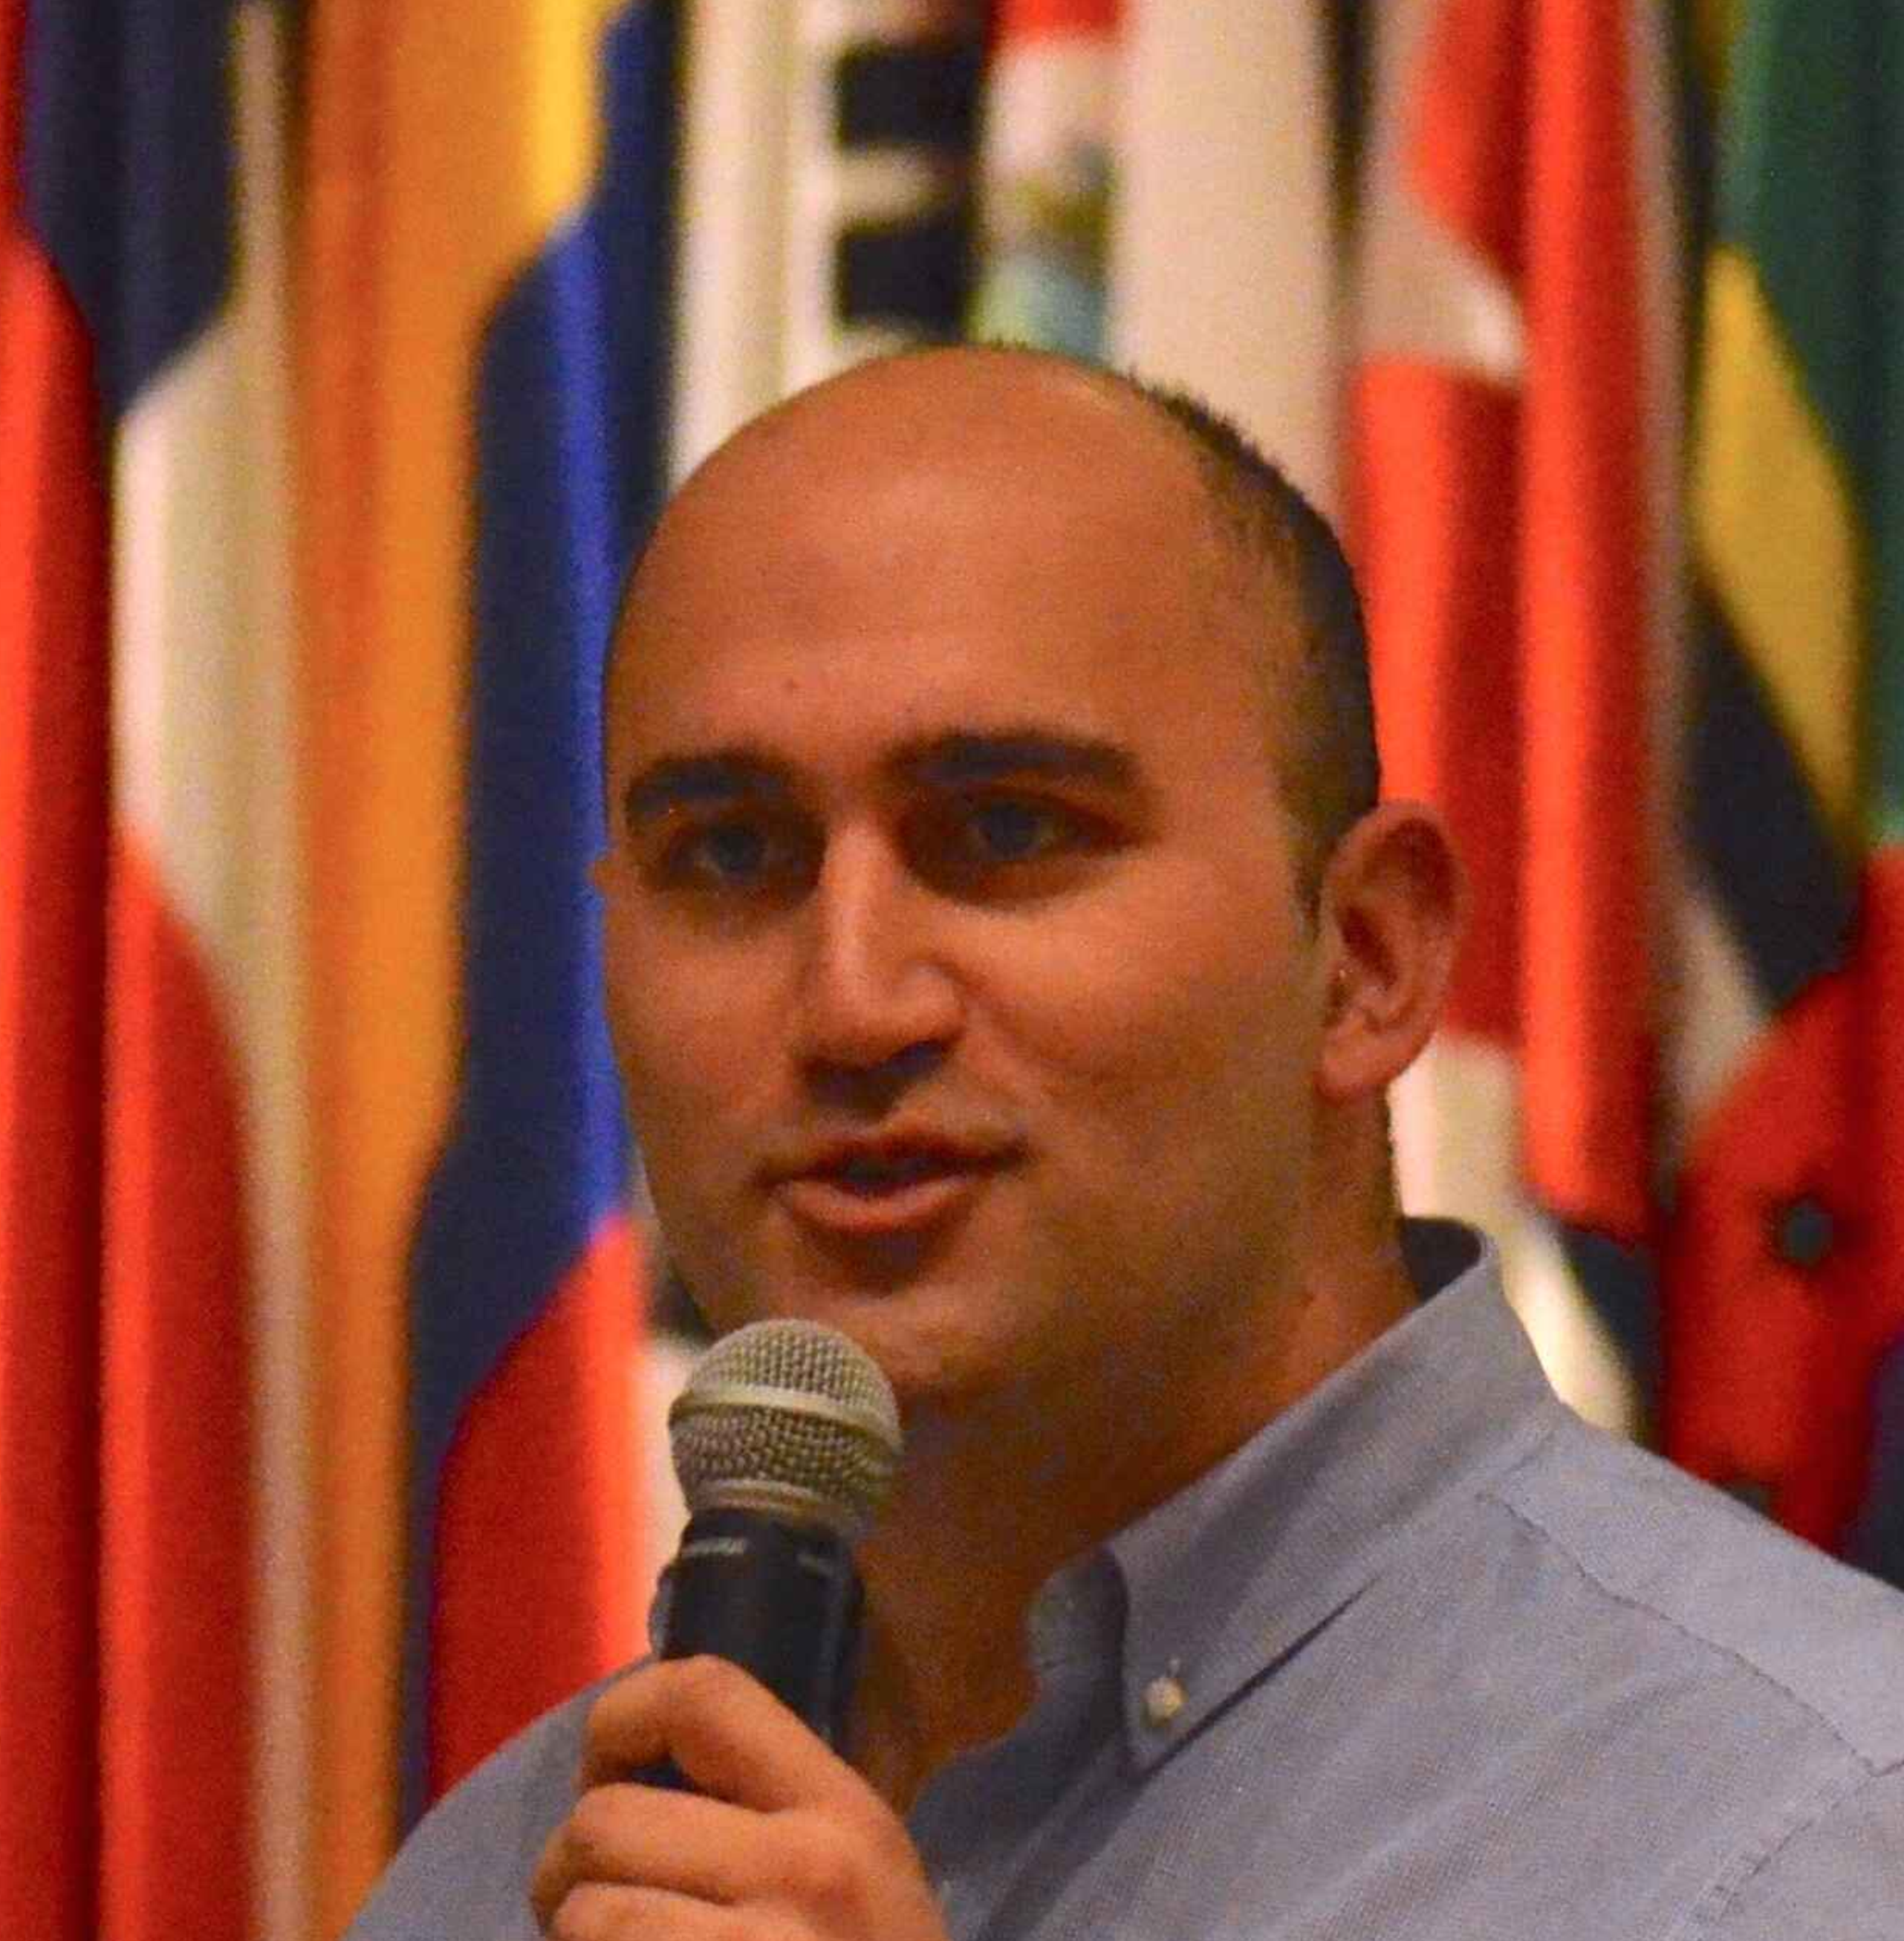
\includegraphics[height=.25\textwidth]{../img/cap0_felipe.pdf}
  \end{textblock}
  \begin{textblock}{7}(14,3)
    
\includegraphics[height=.25\textwidth]{../img/cap0_francisco.jpg}
  \end{textblock}
  \begin{textblock}{7}(14,5.5)
    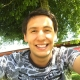
\includegraphics[height=.25\textwidth]{../img/cap0_fernando.jpg}
  \end{textblock}

  \begin{textblock}{7}(14,8)
    
\includegraphics[height=.25\textwidth]{../img/cap0_bruno.jpg}
  \end{textblock}

  \begin{textblock}{7}(14,10.5)
    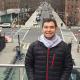
\includegraphics[height=.25\textwidth]{../img/cap0_arie.jpg}
  \end{textblock}

  \begin{textblock}{7}(14,13)
    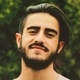
\includegraphics[height=.25\textwidth]{../img/cap0_victor.jpg}
  \end{textblock}



\end{frame}

\section{Inteligencia Artificial}


\begin{frame}{¿Qué es la Inteligencia Artificial?}
\textbf{def. RAE:} Disciplina cientıífica que se ocupa de crear programas
informáticos que ejecutan operaciones comparables a las que realiza
la mente humana, como el aprendizaje o el razonamiento lógico.\\
\vspace{2em}

\textbf{def. Russell \& Norvig:} entender entes inteligentes para aprender
de ellos y construir máquinas inteligentes: interesantes en sí mismos
y útiles en una infinidad de aplicaciones
\vspace{2em}


\textbf{Filosofía de la IA}
\begin{itemize}
  \item La inteligencia es crucial para los seres humanos: a diferencia del resto del reino animal, nosotros no necesitamos evolucionar para adaptarnos.
  \item ¿Puede una máquina actuar inteligentemente?
  \item Si pueden, ¿Cómo es esta inteligencia diferente de la inteligencia humana?
  \item ¿Cuán arraigada en lo humano es la inteligencia?
  \item Inteligencia implica consciencia de sí mismos o tener "mente"
\end{itemize}

\end{frame}

\begin{frame}{Tipos de AI}
    \textbf{Según su naturaleza (J. Searle, 1980):}
    \begin{itemize}
      \item Fuerte: indistinguible de la conciencia humana  
      \item Débil:  indistinguible del actuar humano  
    \end{itemize}
    \vfill
    \textbf{Según su aplicación:}
    \begin{itemize}
      \item General: aplicaciones generales  
      \item Particular: aplicaciones específica  
    \end{itemize}
    \vfill
    \textbf{Definiciones de AI\footnote{(Russel \& Norvig, 2003)}}
    \begin{table}[]
      \scriptsize
      \centering
      \begin{tabular}{|l|c|c|}
        \hline
         & \textbf{Human}     & \textbf{Rational}  \\ \hline
          \textbf{Think}                     & \begin{tabular}[c]{@{}c@{}}``{[}automation of{]} activities associated \\ with human thinking, activities such \\ as descision-making, problem solving,\\  learning" (Bellman, 1978)\end{tabular} & \begin{tabular}[c]{@{}c@{}}``Study of mental faculties \\ through the use of computational \\ models" (Charniak et al., 1985)\end{tabular} \\ \hline
          \multicolumn{1}{|c|}{\textbf{Act}} & \begin{tabular}[c]{@{}c@{}}``The art of creating machines that \\ perform functions that require \\ intelligence when performed \\ by people" (Kurzweil, 1990)\end{tabular} & \begin{tabular}[c]{@{}c@{}}``Study and design of intelligent \\ agents" (Poole et al., 1998)\end{tabular}\\ \hline
        \end{tabular}
      \end{table}
  \end{frame}

\frame[t]{
  \begin{textblock}{1}(1.5,0)
    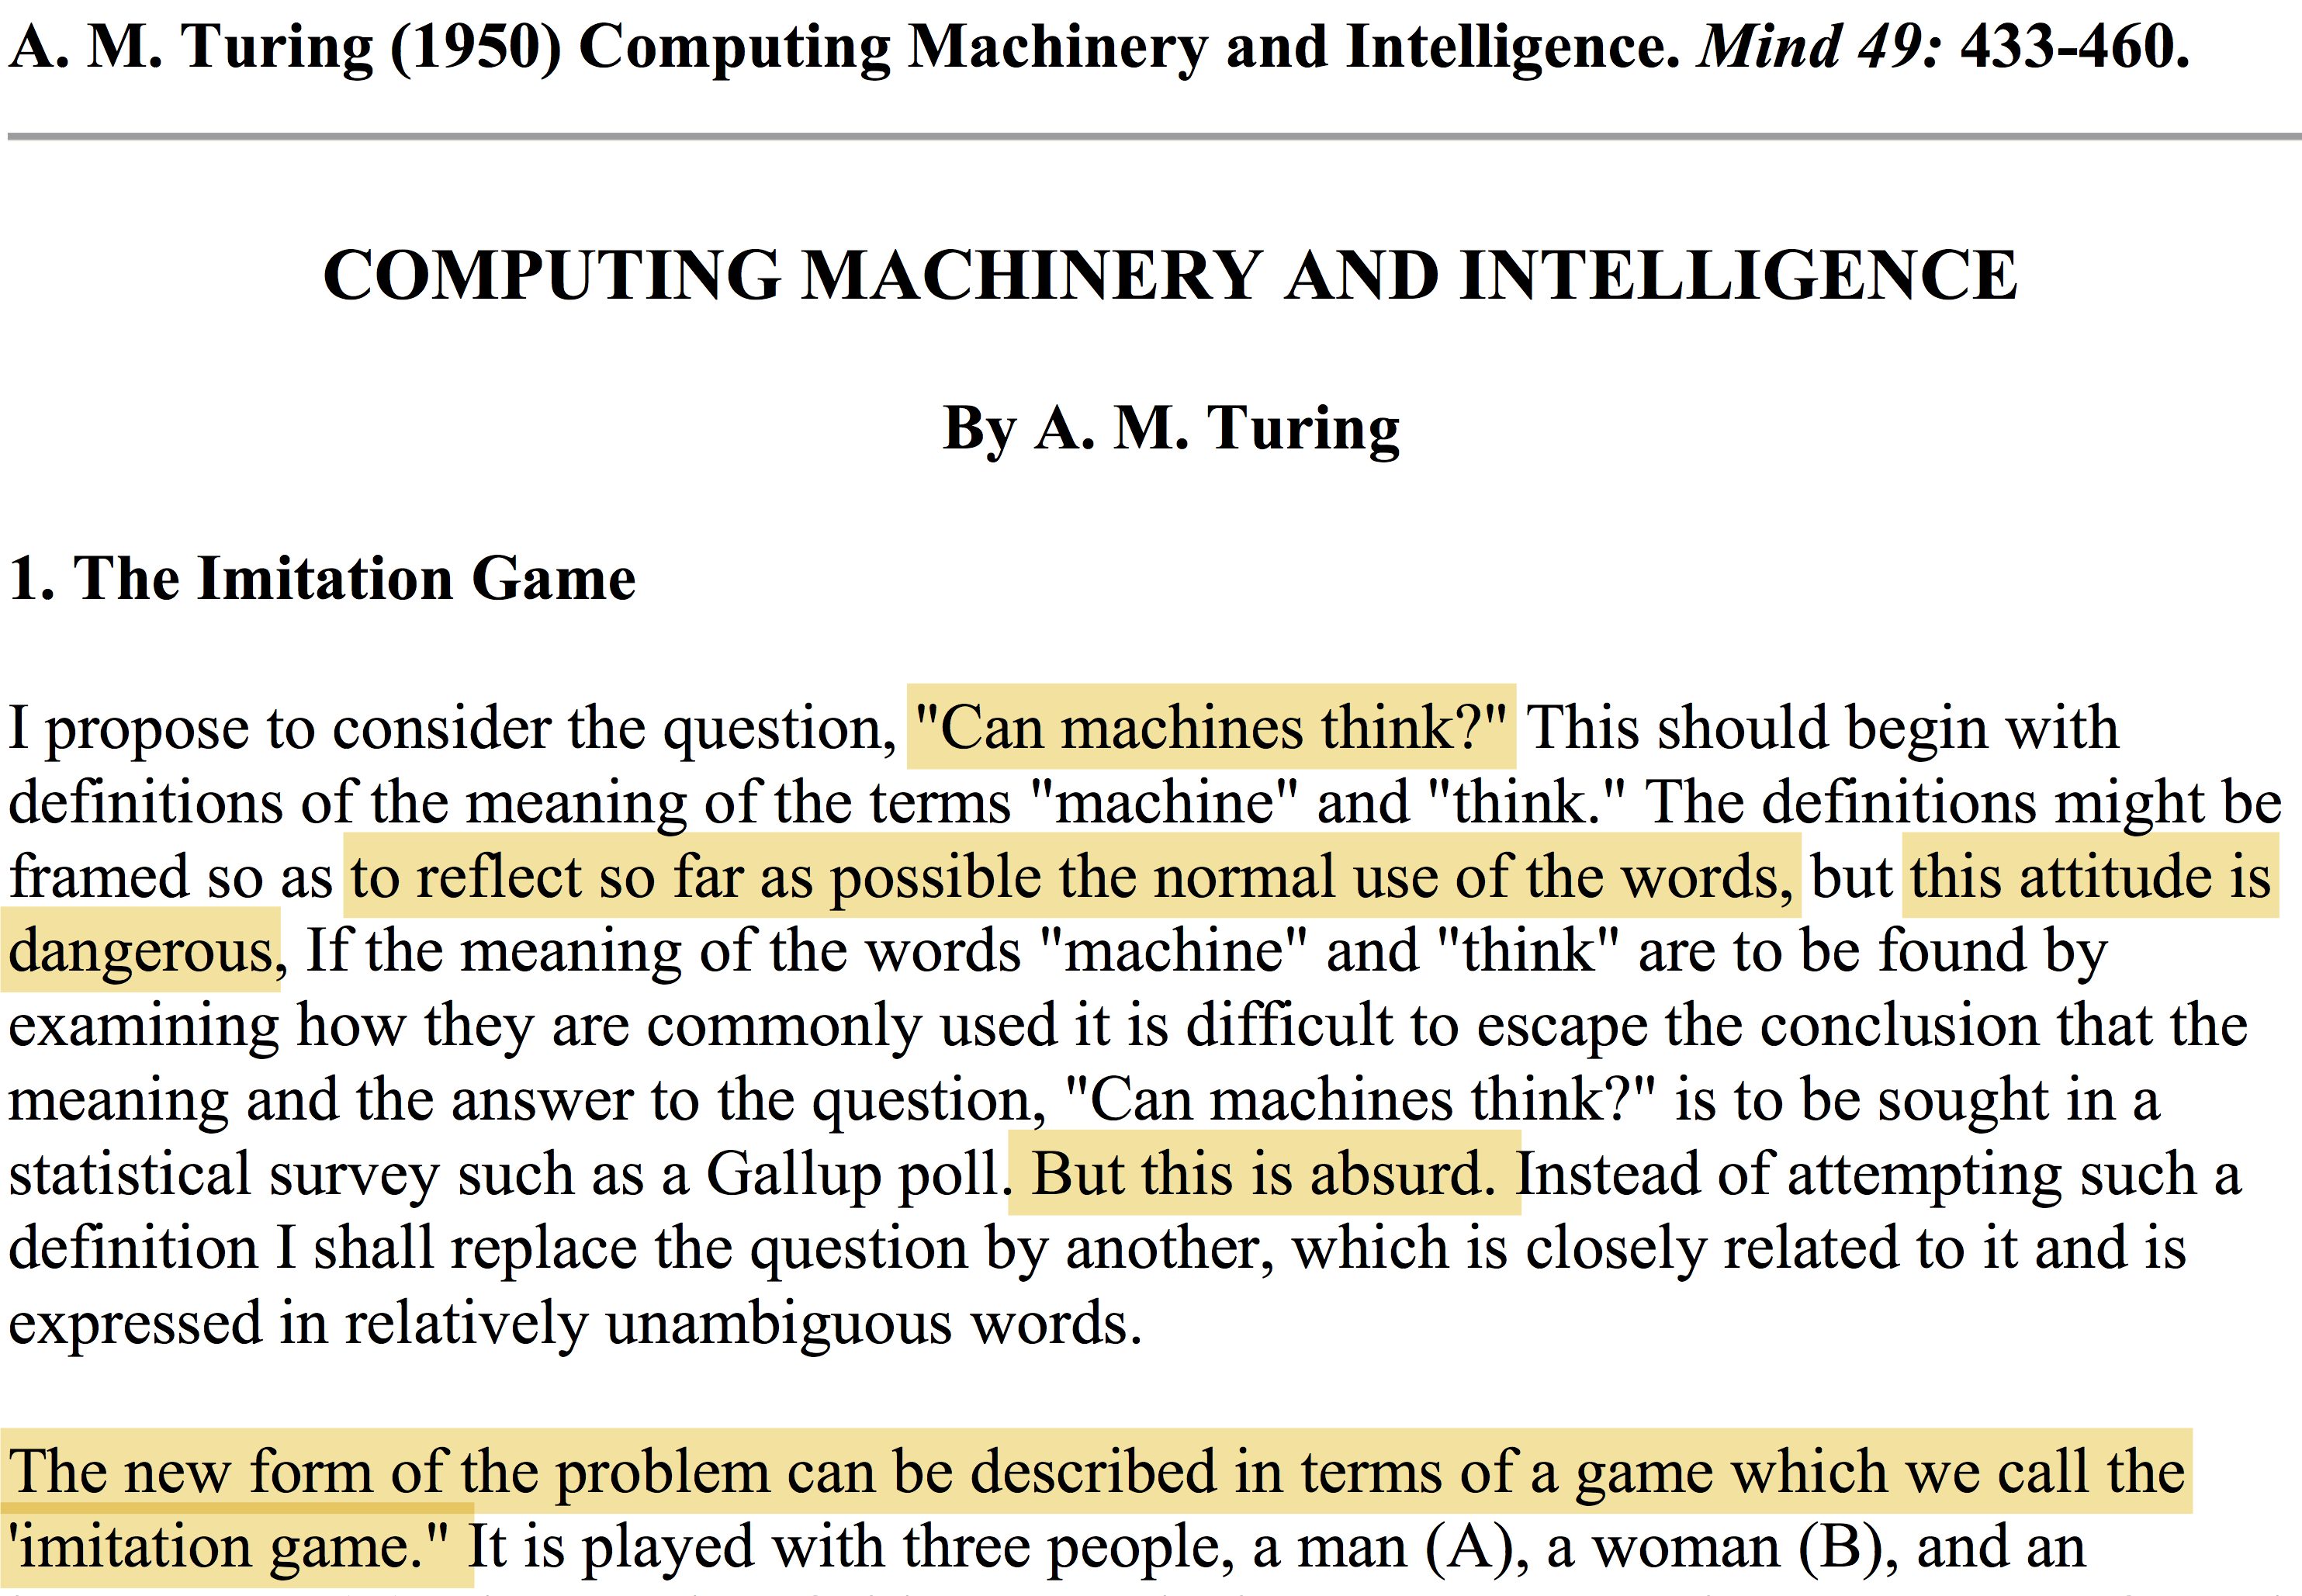
\includegraphics[width=13\textwidth]{../img/cap0_AT}
  \end{textblock}
  \begin{textblock}{1}(13.3,2)
    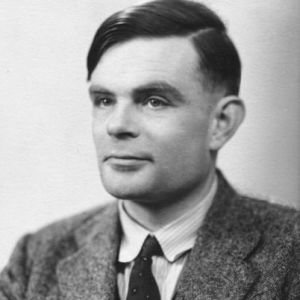
\includegraphics[width=2\textwidth]{../img/cap0_ATp}
  \end{textblock}
  \begin{textblock}{1}(6,12)
    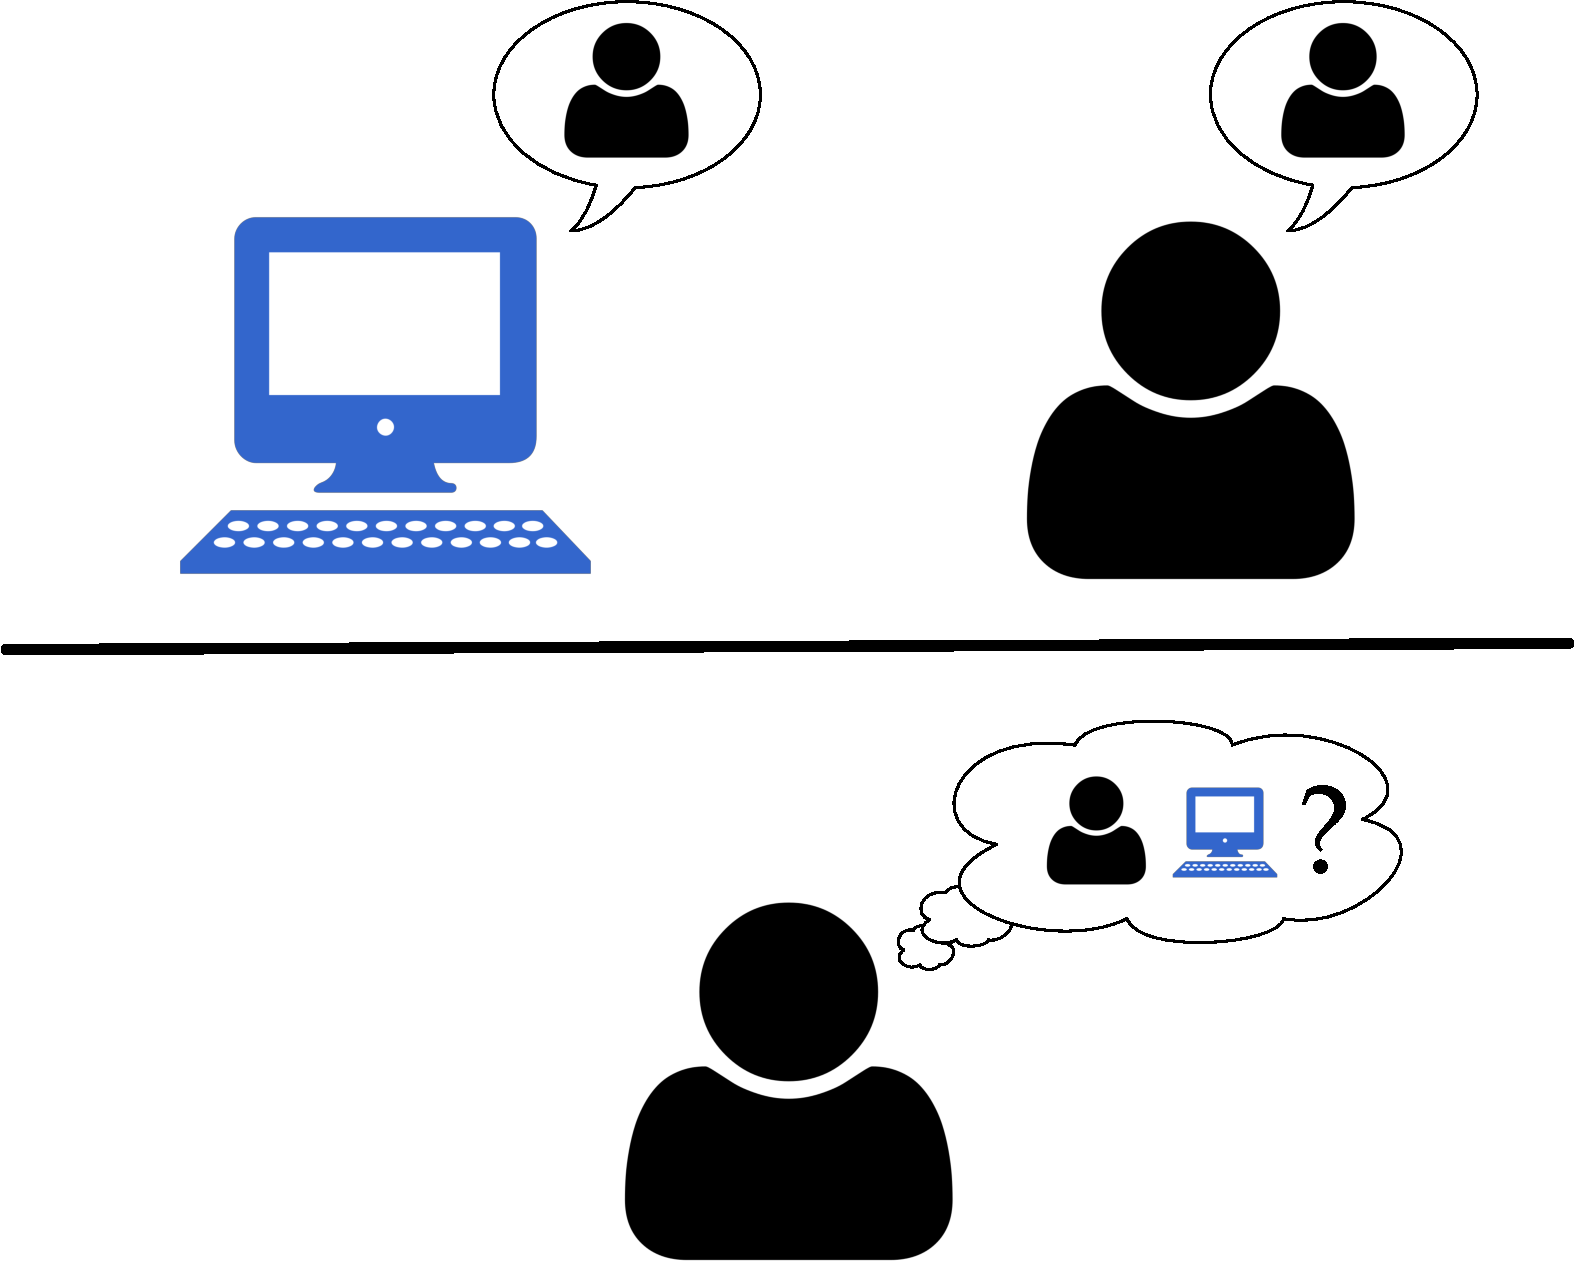
\includegraphics[width=3.5\textwidth]{../img/cap0_turing}
  \end{textblock}
}

\frame[t]{\frametitle{Requerimientos para aprobar el test de Turing}
  \begin{itemize}
    \item \blue{Procesamiento de lenguaje natural:} Habilidad de comunicarse
    \item \blue{Representación de información:} Almacenamiento de \textit{conocimiento}
    \item \blue{Razonamiento:} usar información para concluir
    \item \red{Aprendizaje de máquinas:} construir conocimiento y adaptarse
    \item \blue{Visón computacional$^*$:} percibir el entorno
    \item \blue{Robótica$^*$:} Interactuar con el entorno
  \end{itemize}
  \textbf{$\star$ AM ha dejado de ser una componente exclusiva de IA y se ha convertido en un fin en sí mismo con aplicaciones en variadas disciplinas.}
}

\section{¿Cómo hacemos la inteligencia artificial posible?}

\begin{frame}{GOFAI: Good old fashion artificial intelligence}
  \begin{itemize}
    \item Introduzcamos nuestra forma de actuar en una máquina, esto es conocido como sistemas basados en reglas, sistemas expertos o GOFAI.
    \item Lo bueno: el código de máquinas es interpretable por humanos. 
    \item Lo malo: impracticable más allá de casos de juguete
  \end{itemize}
  \begin{figure}
    \centering
    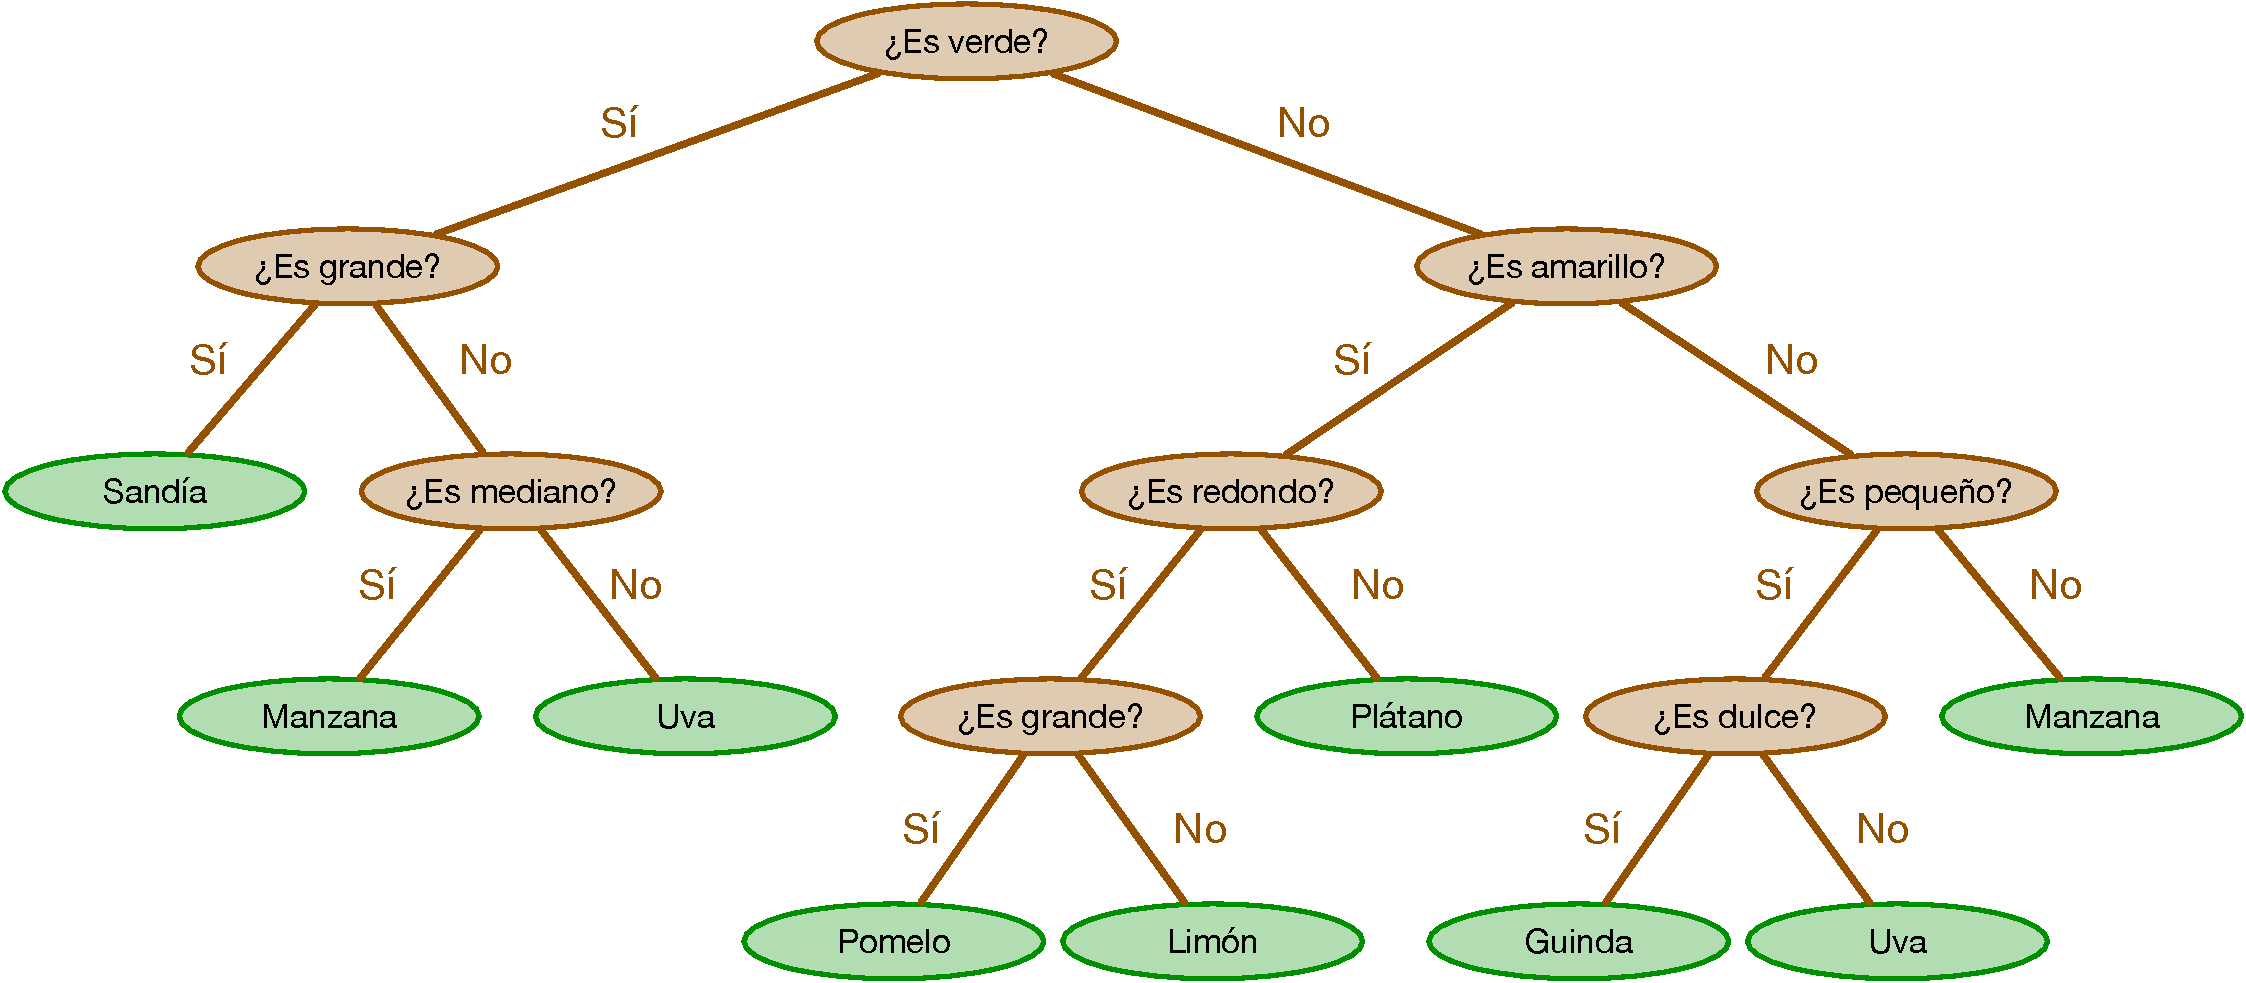
\includegraphics[width=0.9\textwidth]{../img/cap0_arbol}
  \end{figure}
\end{frame}

\begin{frame}{GOFAI para jugar ajedrez}
Un cálculo rápido
  \begin{itemize}
    \item Asumamos que sabemos jugar ajedrez (bien)
    \item El tablero tiene del orden de $10^{43}$ configuraciones distintas
    \item Reglas son: para la posción $P$, mueve la pieza $q$ de la posición C1 a la C2
    \item Asumamos que podemos escribir 10 reglas por segundo, i.e., $315\cdot 10^{6}$ reglas/año
    \item Todos los humanos ($7.5\cdot10^9$) nos ayudan
    \item Nos tomaría \#instrucciones / (velocidad $\cdot$ \#programadores) = $4.2\cdot 10^{24}$ años escribir este programa, es decir, $10^{15}$ veces la edad del universo
  \end{itemize}

  \begin{figure}
    \centering
   % 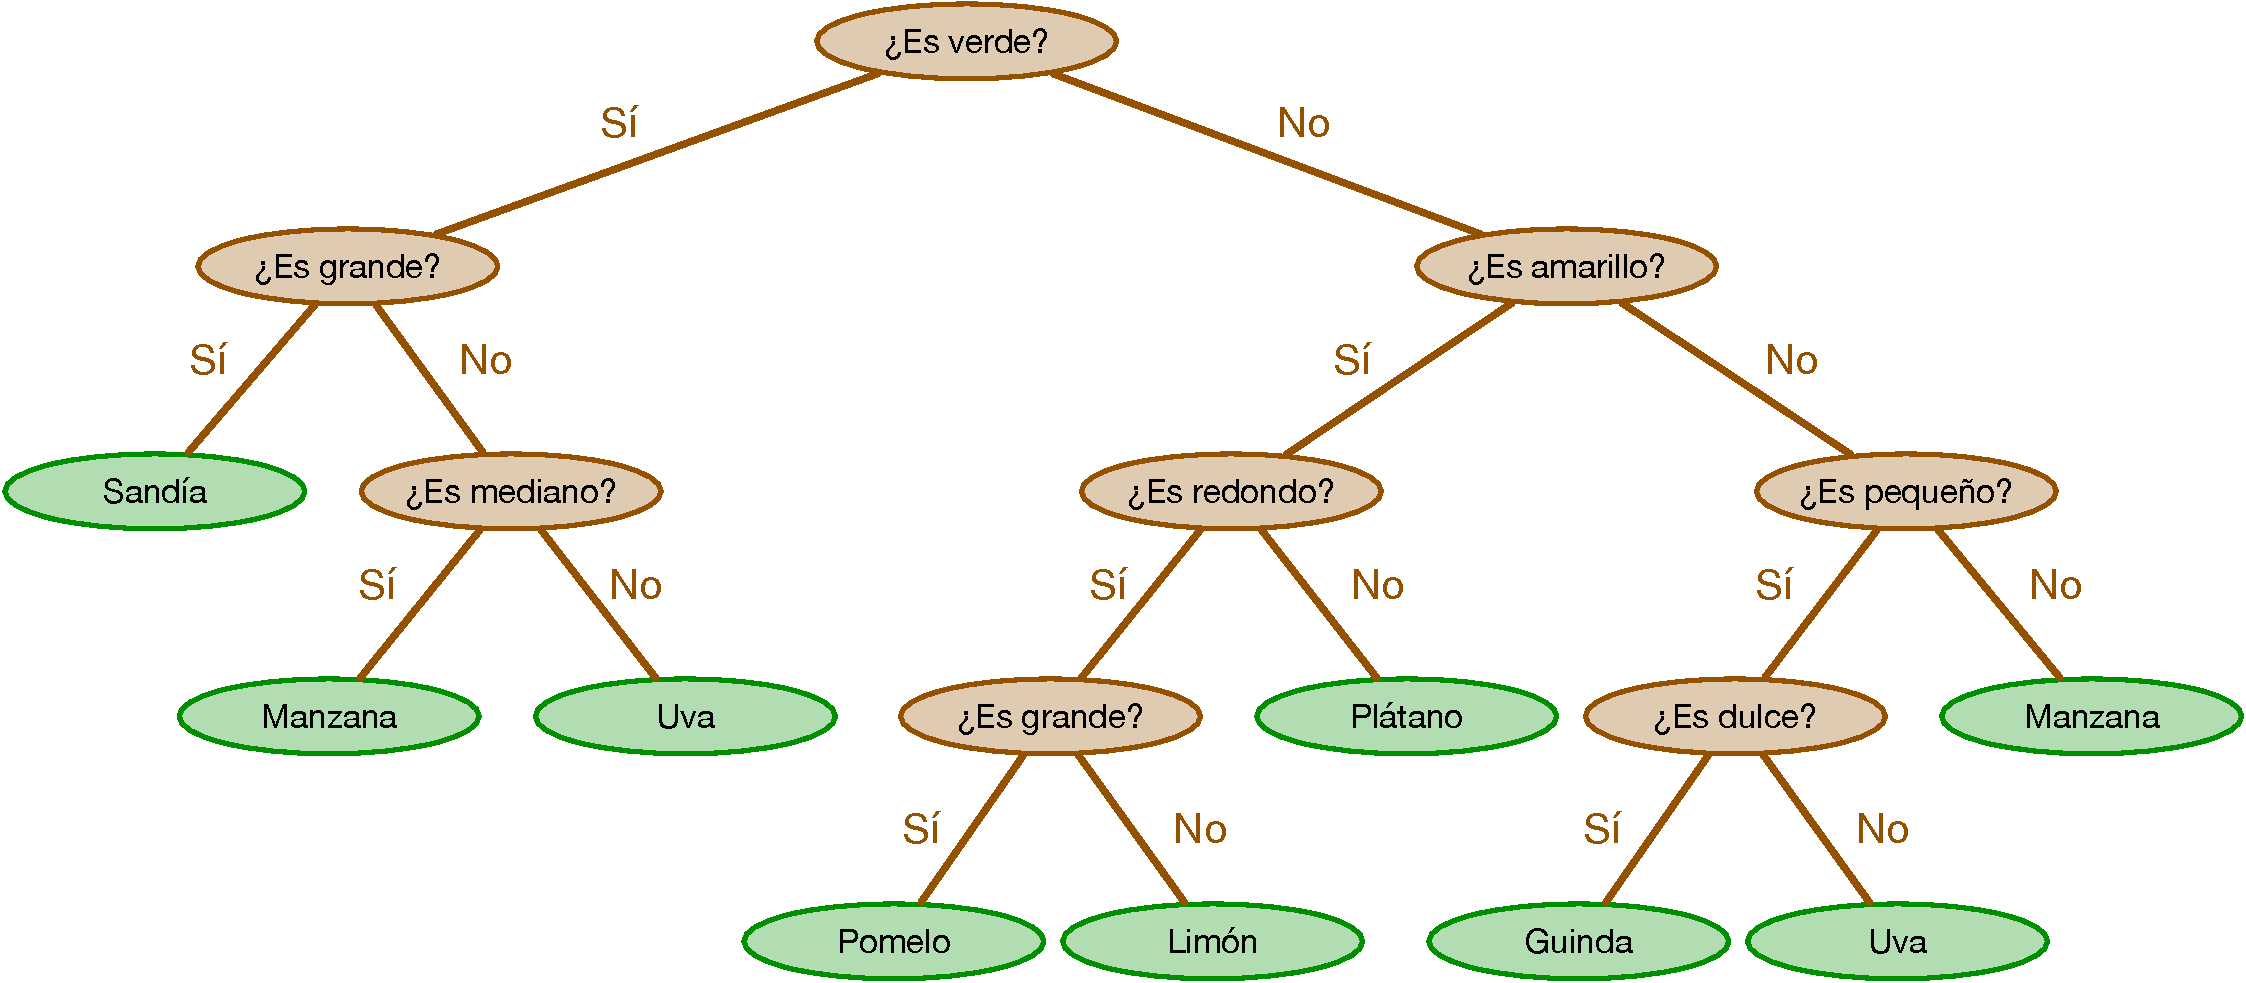
\includegraphics[width=0.9\textwidth]{../img/cap0_arbol}
  \end{figure}
\end{frame}



\begin{frame}{Alternativa: AM para jugar ajedrez}

  \begin{itemize}
    \item En AM, la máquina se programa para aprender a jugar, no para jugar
    \item Consecuentemente, el \emph{output} del proceso no es el juego, es el algoritmo
    \item De esta forma, esperamos que la máquina desarrolle su propia representación
    \item Se fuerza el resultado, no el procedimiento. aprende a jugarAsumamos que sabemos jugar ajedrez (bien)
  \end{itemize}
  \vfill
  \begin{figure}
    \centering
    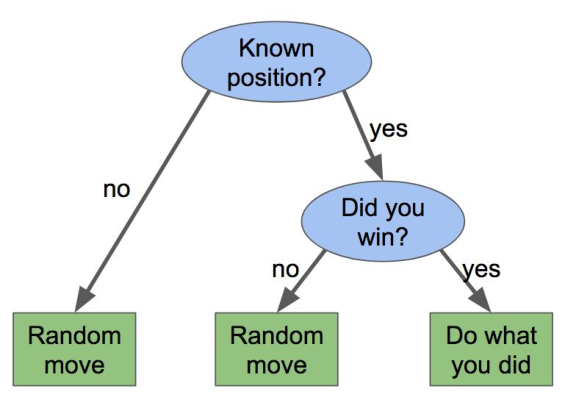
\includegraphics[width=0.45\textwidth]{../img/cap0_chess_ml_diag}\hfill 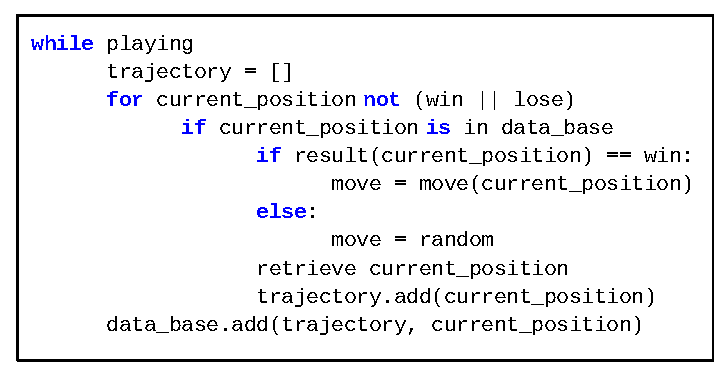
\includegraphics[width=0.52\textwidth]{../img/cap0_chess_ml_code}
  \end{figure}
  \textbf{P: ¿Cómo aprendemos?}\\ R: Buscando 
\end{frame}

\begin{frame}{Tipos de AM}

  \begin{itemize}
    \item Aprendizaje supervisado: 
    Datos de la forma $\{(x_i,y_i)\}_{i=1}^n$, objetivo es encontrar $f$ tal que
    \begin{align}
    x \mapsto y = f(x)
    \end{align}
    \item Aprendizaje no supervisado: Datos de la forma $\{x_i\}_{i=1}^n$, y el objetivo es encontrar patrones en común entre ellos
    \item Aprendizaje reforzado: un \emph{agente}  toma acciones en un \emph{ambiente} con la finalidad de maximizar una función de recompensa
  \end{itemize}

\end{frame}



\begin{frame}{Otros términos}

  \begin{itemize}
    \item Aprendizaje de Máquinas
    \item Inteligencia Artificial
    \item Ciencia de Datos
    \item Minería de Datos
    \item Internet de las Cosas
    \item Big Data
    \item \emph{Analytics}
  \end{itemize}
  \vfill
\textbf{Lectura recomendada:} \href{https://inverseprobability.com/2017/07/17/what-is-machine-learning}{\tt inverseprobability.com/2017/07/17/what-is-machine-learning}

\end{frame}


%Quitar de comentarios apenas se agregue alguna referencia 
\bibliography{../capitulos/referencias} %Bibliografía
\bibliographystyle{apacite}
\end{document} 